\documentclass{article}
\usepackage{amsmath}
\usepackage{physics}
\usepackage{graphicx}
\usepackage{mathrsfs}
\usepackage{amssymb}
\usepackage{microtype}
\usepackage{kotex}
\newcommand{\RN}[1]{%
  \textup{\uppercase\expandafter{\romannumeral#1}}%
}
\begin{document}
\section*{5번 문항 수정안내}
\begin{figure}[!h]
    \centerline{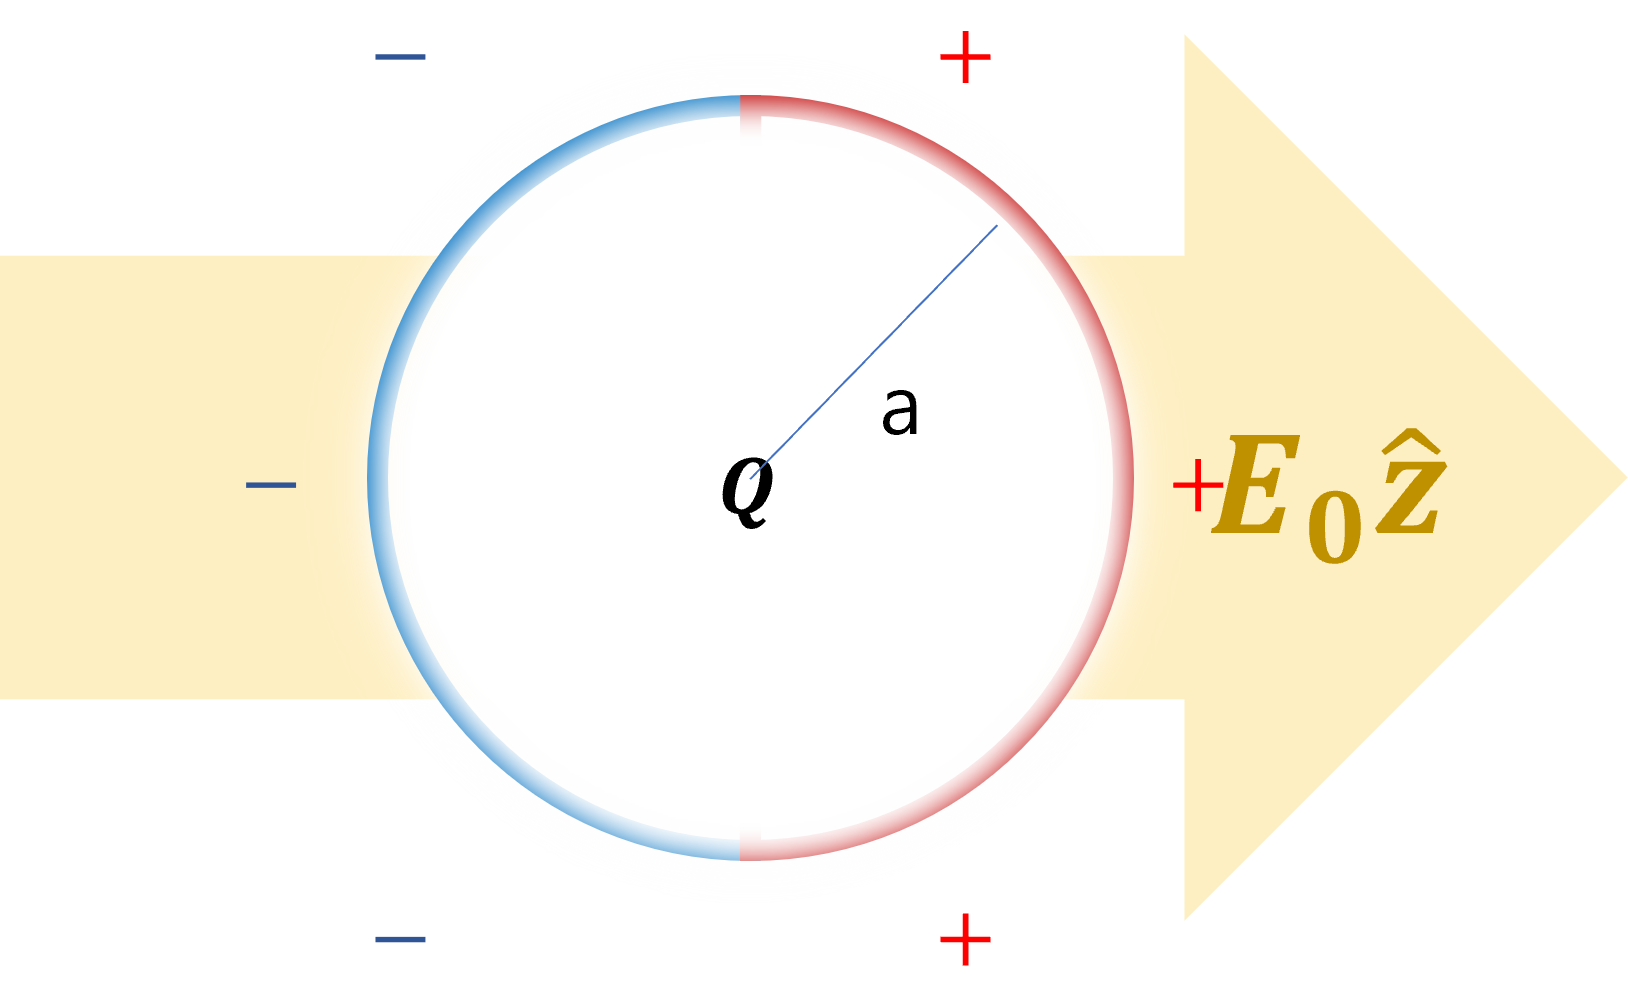
\includegraphics[width=7cm]{EM_Solution_5_edit.png}}
    \caption{균일한 전기장 내의 Q로 charged 된 도체 구}
    \label{figure_1} 
\end{figure}
\begin{equation}
  \varphi(r,\theta) = \sum_{n=0}^{\infty} \bigg( A_nr^n + B_n r^{-(n+1)} P_n(\cos{\theta}) \bigg)
\end{equation}
5번 문제에서는 채점 시 Uniqueness theorem, 즉 도체 구 표면에서 을 올바르게 적용하였는지의 여부를 확인하였고, 이 때 풀이 중 도체 구가 Q로 Charged 되어 있다는 조건을 누락한채 채점을 진행하였습니다.
\\
\\

Q로 Charge된 상태의 구가 아닐 경우 균일한 전기장 내의 도체 구 외부의 전위는 다음과 같이 구해집니다.
\begin{equation}
  \varphi(r,\theta) = E_0 r \cos{\theta} + \frac{E_0 a^3}{r^2} \cos{\theta}
\end{equation}
Q로 Charge 된 상태의 구에서, 전하 Q에 의해 만들어지는 전위 $\frac{Q}{4\pi \epsilon_0 a}$ 를 더하여도 
도체 구 표면에서의 Uniqueness Theorem이 만족됩니다. 이 때의 전위는 다음과 같이 구해집니다.
\begin{equation}
  \varphi(r,\theta) = \frac{Q}{4\pi \epsilon_0 a} + E_0 r \cos{\theta} + \frac{E_0 a^3}{r^2} \cos{\theta}
\end{equation}
\\
채점 기준은 다음과 같이 수정하였습니다. \\ \\
\textbf{
a. 답과 풀이과정을 올바르게 작성하였을 경우 기본 점수 10점,\\\\
b. 답을 올바르게 구하였으나 풀이과정에서 전위의 발산 조건에 의한 $A_n$ 항의 계산 및 일정한 전기장에 의해 생성되는 전위 등,
풀이과정이 충분하지 않을 경우 6점,\\ \\
c. 답이 올바르지 않지만 (2)번 식까지의 논리가 잘 전개된 경우 8점을 부여하였습니다.
}

\section*{7번 문항 수정 안내}
7번 문항의 경우, 배점기준을 조절하였습니다.\\ \\
\textbf{
a. 답과 풀이가 모두 올바른 경우 10점,\\ \\  
b. 답이 올바르지 않지만 풀이가 적절하게 전개된 경우 6점을 부여하였습니다. \\ \\
}

  \end{document}
